%%% - - -   UNCLASSIFIED   - - - %%%

\documentclass[11pt, letterpaper]{article}

\newcommand{\thisdocument}{MILSTD}

\usepackage{format/NGICStyle}        % does everything
\usepackage{format/DurandalBib}      % contains bibliography info
\usepackage{format/NGICGlossary}     % contains glossary info
\usepackage{values/T150ModelValues}   % sets model values

%%% document settings
\graphicspath{{images}}
\newcommand\csvpath{csv}

\makeatletter
\def\input@path{{content}}
\makeatother

\chead{\documentlabel}
\cfoot{\documentlabel\ \\ \thepage}
\presetkeys{todonotes}{disable}{}

%%% document start
\begin{document}

\pagenumbering{roman}

\InDevelopmentfalse

\ifInDevelopment
	\draft
	\linenumbers
	\colorlet{ModelValueColor}{blue!50!cyan}
\fi

%% ============================================================
%%  FRONT MATTER
%% ============================================================

\begin{center}
    \vspace*{0.3in}
    \Huge\textbf{\LARGE\unclass Verification and Validation Plan\\}
    \vspace*{0.15in}
    \Large\textbf{\unclass T-150/TRV-150 Heavy-Lift UAS\\AFSIM Simulation Model v2.0\\}
    \normalsize\textbf{\unclass AFSIM Project 005\\}
    \vspace*{0.3in}
    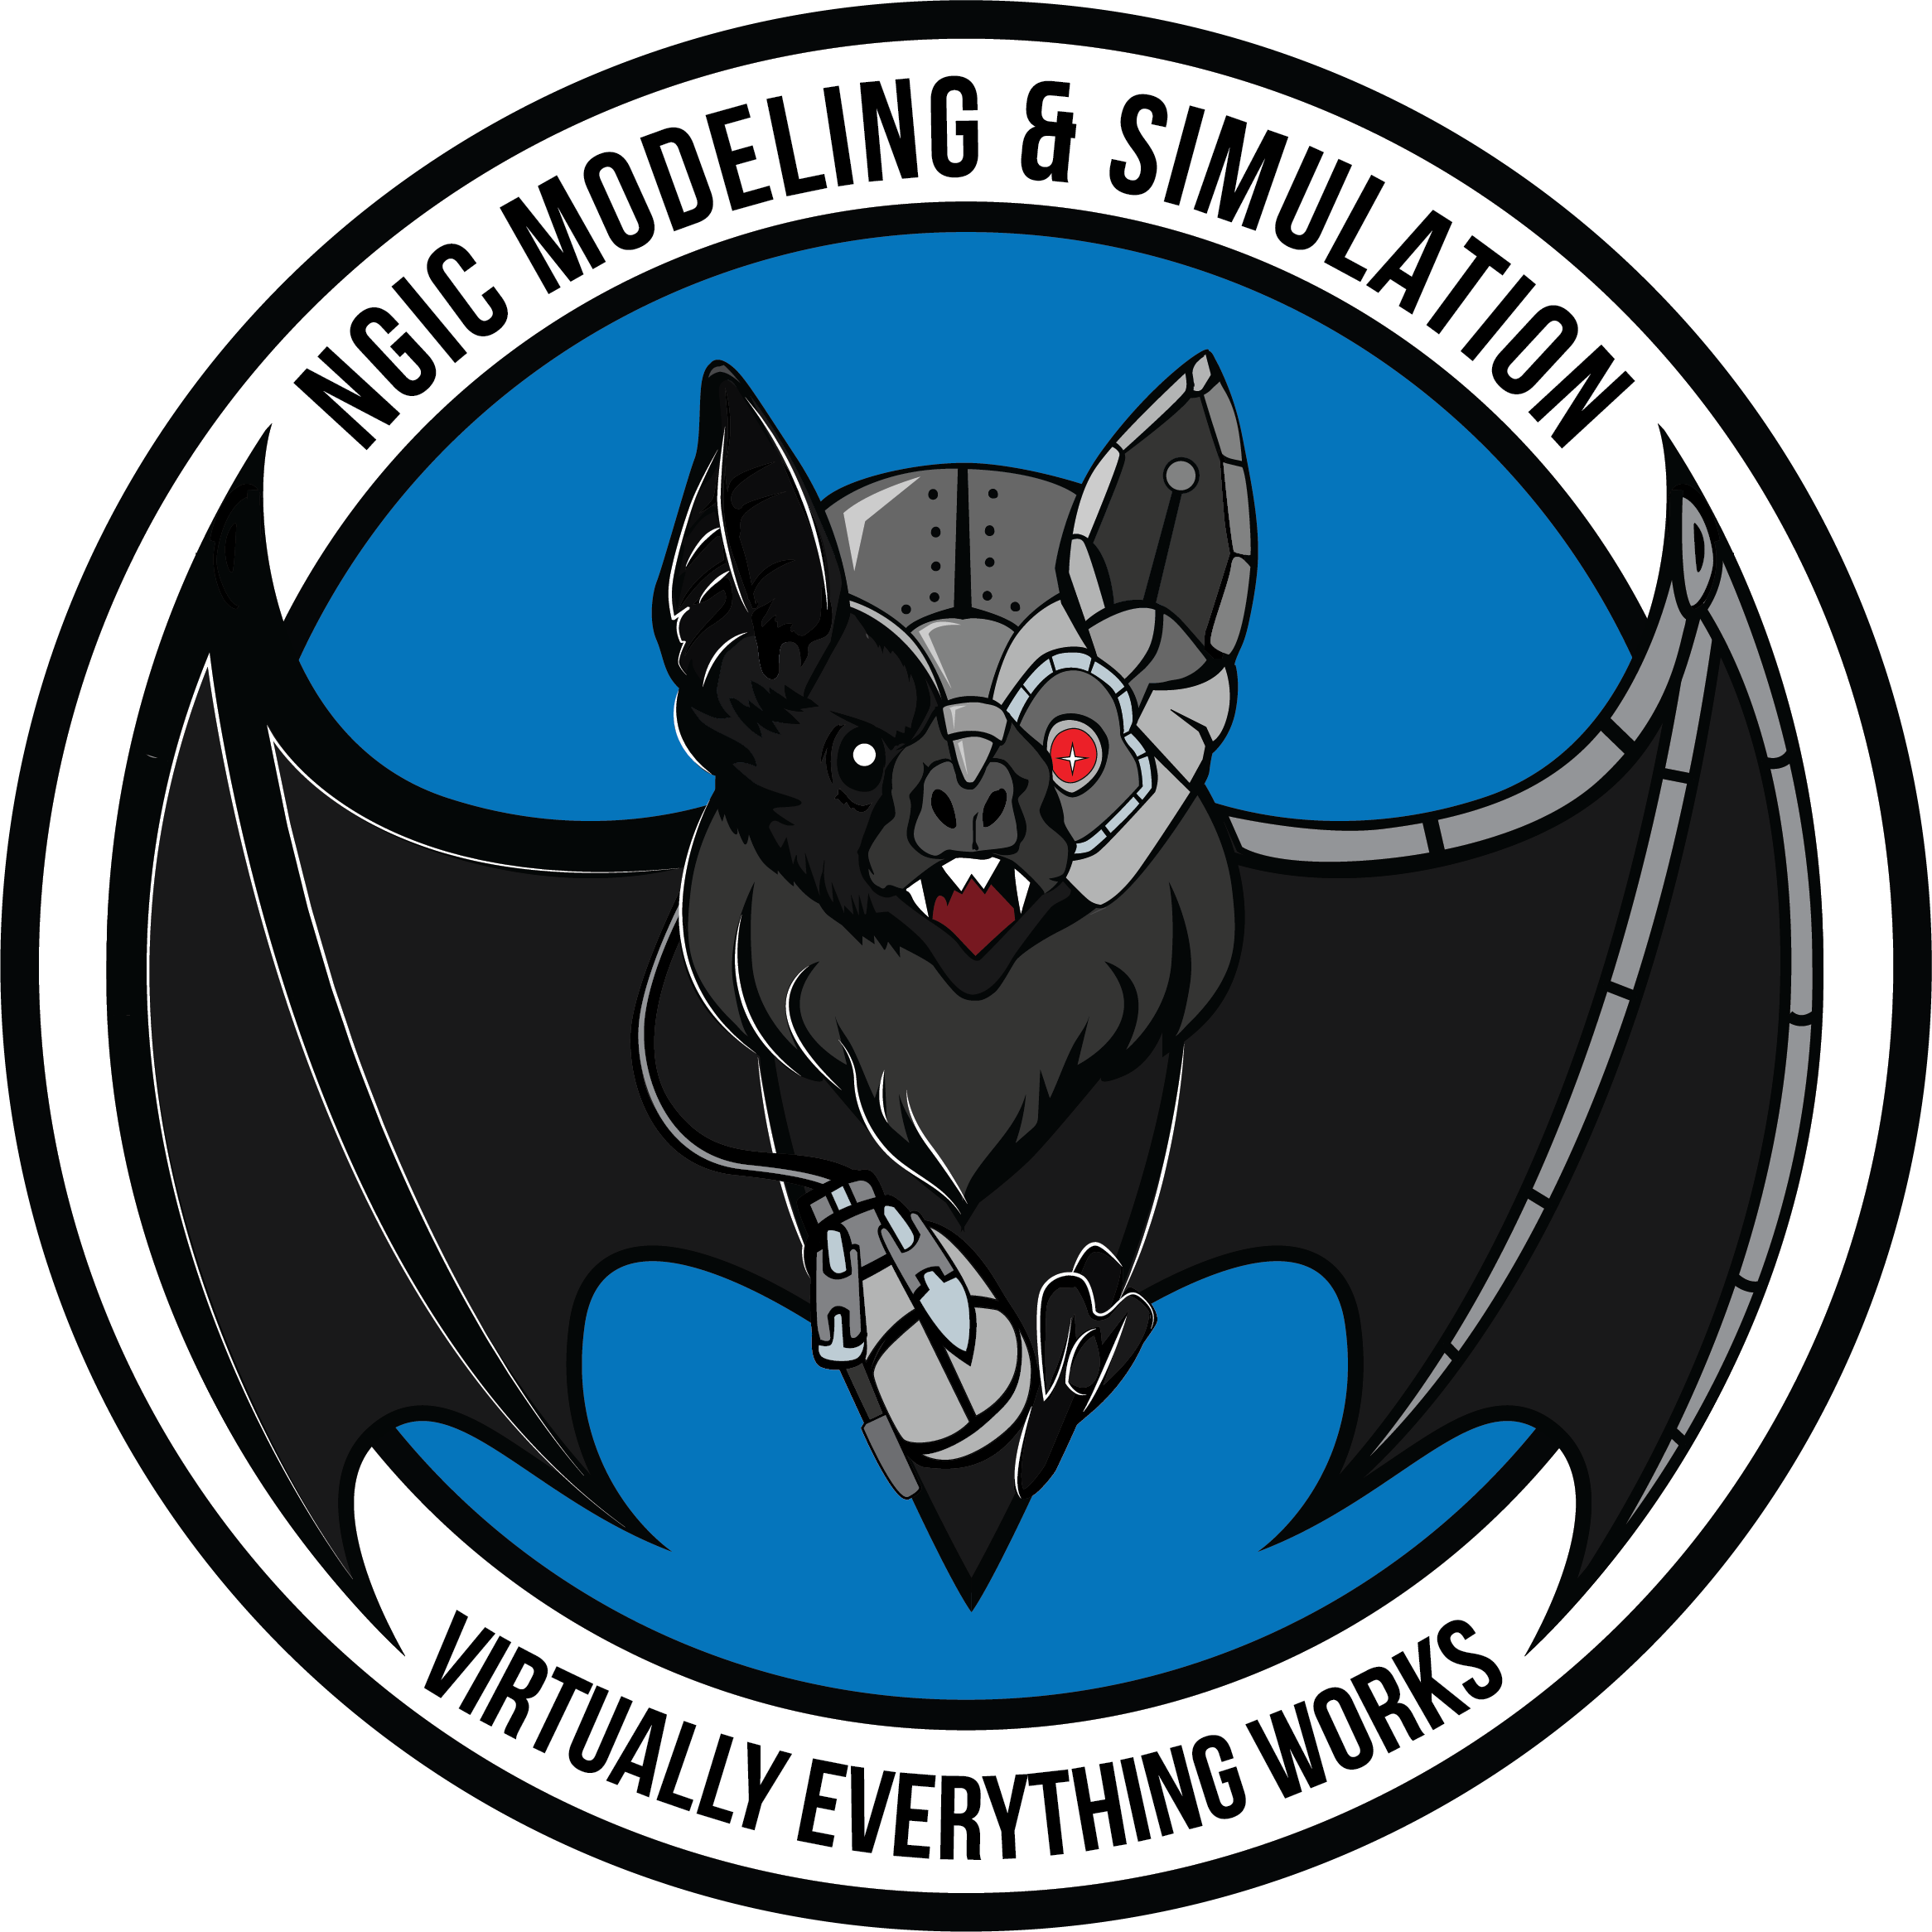
\includegraphics[width=4in]{images/ngic}
    \vspace*{0.1in}
    \Large
    \textbf{Version: 1.0 \\
    Classification: UNCLASSIFIED \\}
\end{center}

\vfill

\tableTwoNow{\unclasslabel}{\unclass Document Information}{vvplan-docinfo}{l,2.5in}{l,3.5in}
{
    Field & Value \\
    Document Version & 1.0 \\
    Date & [PLACEHOLDER - Date] \\
    Classification & UNCLASSIFIED \\
    Sponsoring Organization & [PLACEHOLDER - Organization Name] \\
    Program Manager & [PLACEHOLDER - Name/Title] \\
    Document Preparer & [PLACEHOLDER - Organization/Contract] \\
    Distribution Statement & [PLACEHOLDER - Distribution Statement] \\
    M\&S Name and Version & T-150 UAS AFSIM Plugin Suite v2.0 \\
    V\&V Agent & [PLACEHOLDER - V\&V Agent Organization] \\
    Accreditation Authority & [PLACEHOLDER - Accreditation Authority] \\
}

\pagebreak

%% Record of Changes
\begin{center}
    \begin{tblr}
        {
            colspec     ={|Q[c,0.8in]|Q[c,0.8in]|Q[c,1.5in]|Q[3in]|},
            hline{1-Z}  ={.5pt},
            cell{1}{1}  ={c=4}{halign=l},
            cell{Z}{1}  ={c=4}{halign=r},
            row{2}      ={bg=TableBlue,fg=white,halign=c},
        }
        \unclasslabel\\
        Version & Date     & Author   & Description of Change \\
        1.0     & {[PLACEHOLDER]} & {[PLACEHOLDER]}  & Initial V\&V Plan release per MIL-STD-3022 Appendix B. Covers all five plugins and four test families. \\
        \unclasslabel\\
    \end{tblr}
\end{center}

\vfill\pagebreak

\tableofcontents\thispagestyle{fancy}\pagebreak
\listoftables\thispagestyle{fancy}\pagebreak

\pagenumbering{arabic}
\cfoot{\classlabel\ \\ {Page \thepage\ of \pageref{LastPage}}}


%% ============================================================
%%  EXECUTIVE SUMMARY
%% ============================================================

\section{\unclass Executive Summary}

\unclass This Verification and Validation (V\&V) Plan establishes the framework, requirements, methodology, and acceptance criteria for the formal V\&V of the T-150/TRV-150 Heavy-Lift UAS AFSIM Simulation Model, version 2.0. The plan is prepared in accordance with MIL-STD-3022, ``Documentation of Verification, Validation, and Accreditation (VV\&A) for Models and Simulations'' [2], and supports the accreditation process described in DoDI 5000.61, ``DoD Modeling and Simulation Verification, Validation, and Accreditation'' [1].

\unclass The T-150 UAS AFSIM Plugin Suite v2.0 is a high-fidelity simulation of the T-150/TRV-150 heavy-lift coaxial octocopter, implemented as five custom C++ plugins within the AFSIM 2.2505 framework. The model encompasses 7,736 lines of code distributed across 26 source files, organized into five functional plugins: a physics-based 6DOF mover, a Li-Ion battery model with voltage sag, an electric propulsion system with thermal dynamics, a Vortex Ring State detection and degradation model, and a cable-suspended slung load dynamics model.

\unclass The intended use of this M\&S is to support intelligence analysis of T-150 UAS capabilities, mission planning assessments, Counter-UAS (C-UAS) evaluation, and vulnerability analysis. The model is developed for the intelligence community to answer questions regarding heavy-lift UAS operational performance, flight endurance, payload capacity, and vulnerability conditions.

\unclass This V\&V Plan defines thirteen (13) quantitative requirements with measurable acceptability criteria spanning all five plugin subsystems. Requirements address battery energy conservation, voltage sag fidelity, motor thermal stability, 6DOF position hold and velocity tracking, numerical robustness, VRS state transition accuracy, ground effect modeling, flight endurance, slung load pendulum dynamics, attitude recovery, cruise speed, and maximum payload capacity. Each requirement is traceable to a specific validation test or set of tests.

\unclass The V\&V approach employs a combination of verification techniques (code review, unit testing, integration testing, numerical stability testing) and validation techniques (comparison to manufacturer specifications, comparison to analytical first-principles predictions, energy conservation analysis, and pattern efficiency analysis). Testing is organized into four test families: TF01 (6DOF Physics), TF02 (Battery/Power System), TF03 (VRS Detection), and TF04 (Slung Load Dynamics), comprising a total of sixteen (16) individual tests.

\unclass A key challenge for this V\&V effort is the absence of T-150 flight test data. All validation comparisons are made against manufacturer specifications from open-source product data, analytical predictions derived from first-principles physics (momentum theory, Li-Ion electrochemistry, pendulum dynamics), and published aerodynamic literature. A known gap exists between simulated flight endurance (14.3~minutes) and the manufacturer-stated specification (36~minutes), which has been documented and bounded but not fully resolved.

\pagebreak

%% ============================================================
%%  SECTION 1 -- Problem Statement
%% ============================================================

\section{\unclass Problem Statement}

\subsection{\unclass Intended Use}

\unclass The T-150 UAS AFSIM Plugin Suite v2.0 is intended for the following analytical applications:

\begin{enumerate}
    \item \unclass \textbf{Intelligence Analysis}: Assessing the operational capabilities, performance envelope, and limitations of the T-150/TRV-150 heavy-lift UAS to support intelligence community questions regarding UAS threats. This includes evaluating flight dynamics, payload capacity, energy consumption profiles, and degraded-mode behavior under various operational conditions.
    \item \unclass \textbf{Mission Planning}: Evaluating flight endurance, range, energy consumption, and payload capacity under various mission profiles. The simulation enables analysts to construct mission timelines, estimate fuel (battery) consumption for specific flight profiles, and identify operational constraints for route planning.
    \item \unclass \textbf{Counter-UAS (C-UAS) Assessment}: Providing high-fidelity UAS flight dynamics to support evaluation of detection, tracking, and engagement scenarios against heavy-lift UAS threats.
    \item \unclass \textbf{Vulnerability Analysis}: Analyzing system degradation behavior including Vortex Ring State onset and development, battery depletion effects on voltage and available power, motor thermal limits, slung load instability, and payload-induced performance degradation.
\end{enumerate}

\subsection{\unclass M\&S Overview}

\tableFivNow{\unclasslabel}{\unclass Plugin Suite Overview}{vvplan-plugins}{l,1.2in}{l,1.5in}{l,1.5in}{c,0.5in}{c,0.5in}
{
    Plugin & AFSIM Type Name & Purpose & Files & LOC \\
    rotorcraft\_6dof & Rotorcraft6DOF\_Mover & Physics-based 6DOF flight dynamics with rigid body, rotor model, and flight controller & 8 & $\sim$3,200 \\
    t150\_battery & T150\_BATTERY\_PROCESSOR & Li-Ion battery with SOC tracking, OCV polynomial, voltage sag, internal resistance & 4 & $\sim$1,100 \\
    t150\_propulsion & T150\_PROPULSION\_PROCESSOR & Motor power, thermal dynamics, RPM, ground effect, payload, dynamic power & 4 & $\sim$1,500 \\
    t150\_vrs & T150\_VRS\_PROCESSOR & VRS detection via state machine, margin calculation, lift/control degradation & 4 & $\sim$900 \\
    t150\_slung\_load & T150\_SLUNG\_LOAD\_PROCESSOR & Spherical pendulum slung load, cable tension, resonance detection & 4 & $\sim$1,000 \\
    \textbf{Total} & & & \textbf{26} & \textbf{$\sim$7,736} \\
}

\unclass \textbf{Framework}: AFSIM 2.2505 (Advanced Framework for Simulation, Integration, and Modeling) [7]

\subsection{\unclass M\&S Application}

\unclass The T-150 UAS AFSIM Plugin Suite supports intelligence assessments conducted by [PLACEHOLDER - Organization] regarding the operational capabilities of heavy-lift UAS platforms. Specific analytical products supported include operational performance assessments, flight envelope characterization, energy consumption analysis by mission profile, vulnerability assessments, and C-UAS scenario development.

\subsection{\unclass Accreditation Scope}

\unclass This V\&V Plan supports full model accreditation of the T-150 UAS AFSIM Plugin Suite v2.0 for intelligence analysis use as described in Section 1.1. The accreditation encompasses all five plugins and their integrated behavior within AFSIM 2.2505.

\subsection{\unclass V\&V Scope}

\unclass The V\&V effort encompasses:

\begin{itemize}
    \item \unclass \textbf{Verification}: Confirmation that the model correctly implements the intended physics, algorithms, and data flows as specified in the ADD and UAM. This includes code review, unit-level testing, integration testing, and numerical stability testing.
    \item \unclass \textbf{Validation}: Determination that the model produces results consistent with the intended use by comparison against manufacturer specifications, analytical predictions from first-principles physics, and published literature.
\end{itemize}

\pagebreak

%% ============================================================
%%  SECTION 2 -- Requirements and Acceptability Criteria
%% ============================================================

\section{\unclass M\&S Requirements and Acceptability Criteria}

\tableFivNow{\unclasslabel}{\unclass M\&S Requirements}{vvplan-reqs}{c,0.4in}{l,1.5in}{l,1.5in}{l,1in}{c,0.6in}
{
    Req ID & Requirement Description & Acceptability Criterion & Test Family & Priority \\
    R-001 & Battery SOC shall track energy with high accuracy & Energy error $<$ 0.1\% over full discharge & TF02 & Critical \\
    R-002 & Voltage sag shall match Li-Ion characteristics & Terminal voltage follows OCV minus IR drop & TF02 & High \\
    R-003 & Motor thermal model shall reach stable equilibrium & Temperature converges within 300~s; no runaway & TF02 & High \\
    R-004 & 6DOF mover shall maintain position hold stability & Position drift $<$ 1~m during steady-state hover & TF01 & Critical \\
    R-005 & 6DOF mover shall track commanded velocity & Velocity error $<$ 1~m/s during cruise & TF01 & High \\
    R-006 & All plugins shall maintain numerical stability & No NaN, no divergence, no crashes under extremes & TF01--TF04 & Critical \\
    R-007 & VRS detection shall trigger correct state transitions & CAUTION at margin $<$ 0.8; ONSET at margin $<$ 0.5 & TF03 & High \\
    R-008 & Ground effect shall produce thrust augmentation below 1D & GE factor $>$ 1.0 below 0.76~m AGL; max $\approx$ 1.3 & TF01 & Medium \\
    R-009 & Flight endurance shall fall within calibrated range & Gap documented with identified contributing factors & TF02 & High \\
    R-010 & Slung load pendulum frequency shall match analytic prediction & Measured frequency within 5\% of $f_n = \frac{1}{2\pi}\sqrt{g/L}$ & TF04 & High \\
    R-011 & 6DOF mover shall recover from attitude disturbance & Return to within 5$^\circ$ and 2~m within 10~s & TF01 & Medium \\
    R-012 & Cruise speed shall match manufacturer specification & Steady-state cruise within 1~m/s of 30~m/s & TF01 & High \\
    R-013 & Maximum payload shall be correctly modeled & Model correctly represents 68~kg max payload & TF02 & High \\
}

\pagebreak

%% ============================================================
%%  SECTION 3 -- Assumptions, Capabilities, Limitations, Risks
%% ============================================================

\section{\unclass M\&S Assumptions, Capabilities, Limitations, and Risks/Impacts}

\subsection{\unclass Assumptions}

\tableThrNow{\unclasslabel}{\unclass Model Assumptions}{vvplan-assumptions}{c,0.5in}{l,2.5in}{l,3in}
{
    ID & Assumption & Impact on Results \\
    A-001 & \textbf{Rigid body dynamics}: No structural flexibility or aeroelastic effects & Eliminates high-frequency structural dynamics; acceptable for mission-level analysis \\
    A-002 & \textbf{Standard atmosphere}: Air density at standard sea-level conditions ($\rho$ = 1.225~kg/m$^3$) & Overestimates performance at high altitude; acceptable for low-altitude scenarios \\
    A-003 & \textbf{Symmetric inertia tensor}: Products of inertia are zero & Eliminates cross-coupling terms; valid for symmetric octocopter \\
    A-004 & \textbf{No wind model}: Platform operates in still air & Optimistic endurance and stability results \\
    A-005 & \textbf{Perfect sensors}: All measurements noise-free and lag-free & Overestimates control precision \\
    A-006 & \textbf{Uniform battery cells}: All cells identical in capacity and resistance & Eliminates cell-level failure modes \\
    A-007 & \textbf{Flat terrain}: No terrain elevation model & Ground effect assumes flat ground \\
    A-008 & \textbf{Estimated inertia values}: MOI estimated from geometry, not measured & Affects transient dynamic response \\
}

\subsection{\unclass Capabilities}

\begin{enumerate}
    \item \unclass \textbf{Full 6DOF flight dynamics}: Newton-Euler rigid body physics with quaternion attitude representation, eight individually modeled rotors, PID-based flight controller, and waypoint navigation with spline interpolation.
    \item \unclass \textbf{Battery voltage sag modeling}: SOC-dependent open-circuit voltage via polynomial curve, SOC-dependent internal resistance, quadratic current solution for stable voltage sag calculation.
    \item \unclass \textbf{VRS detection and modeling}: Five-state machine driven by descent rate and forward speed margins, lift degradation factors (down to 0.4x), and control authority degradation factors.
    \item \unclass \textbf{Slung load dynamics}: Two-DOF spherical pendulum model with cable tension calculation, slack and overload detection, resonance detection, and symplectic integration.
    \item \unclass \textbf{Dynamic power modeling}: Flight-state-dependent power calculation incorporating induced power, climb power, parasite drag power, and acceleration power.
    \item \unclass \textbf{Ground effect}: Cheeseman-Bennett approximation with up to 30\% thrust increase at ground level.
    \item \unclass \textbf{Motor thermal dynamics}: First-order thermal model with heat generation, forced convection cooling, and over-temperature warning.
\end{enumerate}

\subsection{\unclass Limitations}

\tableFouNow{\unclasslabel}{\unclass Model Limitations}{vvplan-limitations}{c,0.4in}{l,1.5in}{c,0.8in}{l,3in}
{
    ID & Limitation & Risk & Impact \\
    L-001 & No wind model & Medium & Endurance and range estimates are optimistic \\
    L-002 & VRS is informational only & Medium & VRS factors computed but do not modify flight dynamics \\
    L-003 & Slung load forces do not feed back to mover & Medium & Pendulum forces published but do not alter trajectory \\
    L-004 & Flight endurance gap (14.3 vs.\ 36~min) & Medium & Direct time-based analysis requires calibration factor \\
    L-005 & Constant air density & Low & Performance does not degrade with altitude \\
    L-006 & No structural failure modes & Low & Single-point failures not assessable \\
}

\subsection{\unclass Risks/Impacts}

\tableFouNow{\unclasslabel}{\unclass V\&V Risks}{vvplan-risks}{l,2in}{c,0.7in}{c,0.7in}{l,2.5in}
{
    Risk & Probability & Impact & Mitigation \\
    \textbf{Endurance gap} limits time-based analysis & High & Medium & Document calibration factor ($\approx$2.5x); recommend speed-based metrics \\
    \textbf{No flight test data} for direct validation & High & Medium & Multiple independent validation approaches; classify confidence levels \\
    \textbf{Estimated parameters} may not match actual T-150 & Medium & Medium & Sensitivity analysis on key parameters; bound uncertainty ranges \\
    \textbf{Self-testing} reduces V\&V independence & Medium & Low & Objective quantitative criteria; recommend independent review \\
}

\pagebreak

%% ============================================================
%%  SECTION 4 -- V&V Methodology
%% ============================================================

\section{\unclass V\&V Methodology}

\subsection{\unclass V\&V Approach}

\unclass \textbf{Verification} establishes that the code correctly implements the intended algorithms and physics. Verification activities include:
\begin{itemize}
    \item \unclass Peer code review of algorithms against design documentation
    \item \unclass Unit-level numerical checks of mathematical functions
    \item \unclass Integration testing of inter-plugin data flow via AuxData
    \item \unclass Boundary and stress testing for numerical robustness
\end{itemize}

\unclass \textbf{Validation} establishes that the model's outputs are consistent with real-world behavior within acceptable tolerances. Validation employs three complementary approaches:
\begin{enumerate}
    \item \unclass \textbf{Comparison to manufacturer specifications}: Cruise speed, maximum payload, battery capacity, and stated flight time [11]
    \item \unclass \textbf{Comparison to analytical predictions}: Hover power from momentum theory, pendulum natural frequency, VRS onset boundaries [9, 10]
    \item \unclass \textbf{Energy conservation and internal consistency}: Verifying that energy in equals energy out and that state transitions occur at predicted thresholds
\end{enumerate}

\subsection{\unclass Verification Tasks}

\subsubsection{\unclass Code Review}

\unclass All 26 source files across the five plugins shall be reviewed for correctness of physics equations, proper unit conversions, numerical guard conditions, proper initialization, and correct AFSIM API usage.

\tableThrNow{\unclasslabel}{\unclass Code Review Scope}{vvplan-codereview}{l,1.5in}{l,2in}{l,2.5in}
{
    Plugin & Source Files & Key Algorithms to Review \\
    rotorcraft\_6dof & RigidBody6DOF, RotorModel, Mover, MathUtils & Quaternion integration, Newton-Euler, rotor thrust/torque, PID controllers \\
    t150\_battery & BatteryProcessor & OCV polynomial, quadratic current solver, SOC integration \\
    t150\_propulsion & PropulsionProcessor & Momentum theory thrust, efficiency curves, thermal dynamics, ground effect \\
    t150\_vrs & VRSProcessor & VRS margin calculation, state machine transitions \\
    t150\_slung\_load & SlungLoadProcessor & Pendulum equations of motion, symplectic integration, cable tension \\
}

\subsubsection{\unclass Unit-Level Testing}

\unclass Unit-level tests verify individual mathematical functions in isolation: OCV polynomial evaluation, quadratic current solver, thrust coefficient calculation, pendulum angular acceleration, VRS margin calculation, and quaternion operations.

\subsubsection{\unclass Integration Testing}

\unclass Integration tests verify inter-plugin communication and data consistency: propulsion-to-battery power flow, mover-to-VRS velocity flow, mover-to-slung-load acceleration flow, and battery SOC depletion rate consistency.

\subsubsection{\unclass Numerical Stability Testing}

\unclass Stress tests under boundary conditions: zero payload, maximum payload, overload ($>$68~kg), battery SOC at 0\% and 100\%, extreme descent rates ($>$8~m/s), near-zero altitude, and extreme time step sizes.

\subsection{\unclass Validation Tasks}

\subsubsection{\unclass Manufacturer Specification Comparison}

\tableThrNow{\unclasslabel}{\unclass Manufacturer Specification Comparison}{vvplan-mfgcomp}{l,2in}{l,2in}{l,2in}
{
    Parameter & Manufacturer Value & Acceptance Criterion \\
    Cruise speed & 30~m/s & Within 1~m/s \\
    Maximum payload & 68~kg (150~lbs) & Exact match (model parameter) \\
    Battery capacity & $\sim$7~kWh & Exact match (model parameter) \\
    Battery configuration & 13S Li-Ion & Exact match (model parameter) \\
    Flight time & 36~minutes & Document gap; provide calibration \\
    MTOW & 123~kg & Within 5~kg \\
}

\subsubsection{\unclass Analytical Prediction Comparison}

\tableFouNow{\unclasslabel}{\unclass Analytical Predictions}{vvplan-analytic}{l,1.5in}{l,2in}{l,1.2in}{l,1.3in}
{
    Prediction & Analytical Formula & Expected Value & Acceptance Criterion \\
    Hover power & $P = T \cdot v_i$, where $v_i = \sqrt{T / (2\rho A)}$ & $\sim$17--20~kW & Within 15\% \\
    Pendulum frequency & $f_n = \frac{1}{2\pi}\sqrt{g/L}$ & 0.223~Hz ($L$=5~m) & Within 5\% \\
    VRS onset descent rate & $v_\text{desc}$ approaching $v_i$ & $\sim$4~m/s & Correct detection \\
    Ground effect factor & $1 / (1 - (R/4h)^2)$ & $\sim$1.3 at $h = R/4$ & Within 10\% \\
    Bank angle thrust loading & $T = mg / \cos\phi$ & 1.15x at 30$^\circ$ & Within 5\% \\
}

\subsubsection{\unclass Energy Conservation Validation}

\unclass Energy conservation testing verifies that total energy consumed equals the integral of power over time. Acceptance criterion: energy balance error $<$ 0.1\%.

\subsubsection{\unclass Pattern Efficiency Analysis}

\unclass Flight pattern efficiency analysis validates that relative energy cost of different maneuver patterns follows physically expected trends: straight-line (baseline) $<$ sawtooth $<$ sine wave $<$ cycloid $<$ square wave.

\subsection{\unclass Test Families}

\subsubsection{\unclass TF01: 6DOF Physics (5 Tests)}

\tableFouNow{\unclasslabel}{\unclass TF01: 6DOF Physics Tests}{vvplan-tf01}{c,0.6in}{l,1.3in}{c,0.5in}{l,3.5in}
{
    Test ID & Test Name & Req & Description \\
    TF01-01 & Hover Stability & R-004 & Command hover at fixed position for 60~s. Measure drift after 10~s transient. Verify drift $<$ 1~m. \\
    TF01-02 & Cruise Velocity Tracking & R-005, R-012 & Command cruise at 30~m/s. Measure achieved speed. Verify error $<$ 1~m/s. \\
    TF01-03 & Attitude Recovery & R-011 & Apply asymmetric disturbance. Verify return to level hover within 10~s. \\
    TF01-04 & Ground Effect Validation & R-008 & Hover at 0.2, 0.5, 1.0, 2.0~m AGL. Compare GE factor to Cheeseman-Bennett. \\
    TF01-05 & Numerical Robustness & R-006 & Execute extreme maneuver sequences. Verify no NaN or divergence. \\
}

\subsubsection{\unclass TF02: Battery/Power System (5 Tests)}

\tableFouNow{\unclasslabel}{\unclass TF02: Battery/Power System Tests}{vvplan-tf02}{c,0.6in}{l,1.3in}{c,0.5in}{l,3.5in}
{
    Test ID & Test Name & Req & Description \\
    TF02-01 & Energy Conservation & R-001 & Full discharge from 100\% to 0\% SOC. Verify energy error $<$ 0.1\%. \\
    TF02-02 & Voltage Sag & R-002 & Hover at multiple SOC levels. Verify $V = OCV - IR$ relationship. \\
    TF02-03 & Motor Thermal Equilibrium & R-003 & Sustained hover for 300~s. Verify temperature convergence. \\
    TF02-04 & Flight Endurance & R-009 & Hover until depletion. Document endurance and gap analysis. \\
    TF02-05 & Payload Capacity & R-013 & Configure payload at 0, 34, 68, 75~kg. Verify overload flag at 75~kg. \\
}

\subsubsection{\unclass TF03: VRS Detection (3 Tests)}

\tableFouNow{\unclasslabel}{\unclass TF03: VRS Detection Tests}{vvplan-tf03}{c,0.6in}{l,1.5in}{c,0.5in}{l,3.3in}
{
    Test ID & Test Name & Req & Description \\
    TF03-01 & VRS State Transitions & R-007 & Controlled descent at increasing rates with zero forward speed. Verify state transitions. \\
    TF03-02 & Forward Speed Immunity & R-007 & Descent at 5~m/s with forward speeds of 0, 2, 5, 10~m/s. Verify VRS suppression above 5~m/s. \\
    TF03-03 & Numerical Robustness (VRS) & R-006 & Extreme descent rates and rapid transitions. Verify no stuck states. \\
}

\subsubsection{\unclass TF04: Slung Load Dynamics (3 Tests)}

\tableFouNow{\unclasslabel}{\unclass TF04: Slung Load Dynamics Tests}{vvplan-tf04}{c,0.6in}{l,1.5in}{c,0.5in}{l,3.3in}
{
    Test ID & Test Name & Req & Description \\
    TF04-01 & Pendulum Frequency & R-010 & 5~m cable, 25~kg load. Apply impulse. Verify frequency within 5\% of 0.223~Hz. \\
    TF04-02 & Load State Transitions & R-010 & Verify DETACHED $\rightarrow$ ATTACHED $\rightarrow$ SWINGING $\rightarrow$ RESONANCE transitions. \\
    TF04-03 & Numerical Robustness & R-006 & Extreme cable lengths (0.5--20~m), masses (1--55~kg), rapid accelerations. \\
}

\pagebreak

%% ============================================================
%%  SECTION 5 -- V&V Issues
%% ============================================================

\section{\unclass V\&V Issues}

\subsection{\unclass Absence of Flight Test Data}

\unclass No T-150 flight test data is available for direct model-versus-test validation. All validation is performed against manufacturer specifications, analytical predictions, and published literature.

\unclass \textbf{Impact}: Validation confidence is bounded by the quality of analytical predictions and manufacturer specifications.

\unclass \textbf{Mitigation}: Multiple independent validation approaches are used. Confidence levels are explicitly stated per capability.

\subsection{\unclass Flight Endurance Gap}

\unclass Simulated endurance of 14.3~minutes significantly differs from the 36-minute manufacturer specification. Contributing factors include hover power assumptions and absence of manufacturer-specific motor efficiency data.

\unclass \textbf{Impact}: Direct use of simulated endurance for absolute time-based analysis produces non-conservative results.

\unclass \textbf{Mitigation}: The gap is documented with a calibration factor. Analysts instructed to use relative metrics.

\subsection{\unclass Estimated Parameters}

\unclass Several parameters are estimated from class-level data rather than measured from the actual T-150: moments of inertia, motor thermal mass, battery internal resistance, and drag coefficient.

\unclass \textbf{Impact}: Transient dynamics may differ from actual T-150 behavior.

\unclass \textbf{Mitigation}: Sensitivity analysis recommended. Parameter values documented with sources.

\subsection{\unclass No Independent V\&V Agent}

\unclass V\&V is performed by the model developer rather than by an independent agent, introducing potential confirmation bias.

\unclass \textbf{Impact}: Reduced independence may limit accreditation authority's confidence.

\unclass \textbf{Mitigation}: All activities use objective, quantitative criteria defined in advance. Results fully documented for independent review.

\pagebreak

%% ============================================================
%%  SECTION 6 -- Key Participants
%% ============================================================

\section{\unclass Key Participants}

\tableFouNow{\unclasslabel}{\unclass Key Participants}{vvplan-participants}{l,1.8in}{l,1.5in}{l,1.5in}{l,1.5in}
{
    Role & Organization & Individual & Responsibility \\
    V\&V Agent & [PLACEHOLDER] & [PLACEHOLDER] & Plan, execute, and document V\&V activities \\
    M\&S Developer & [PLACEHOLDER] & [PLACEHOLDER] & Develop and maintain the plugin suite \\
    Accreditation Authority & [PLACEHOLDER] & [PLACEHOLDER] & Review V\&V results and make accreditation determination \\
    M\&S Proponent & [PLACEHOLDER] & [PLACEHOLDER] & Define intended use and analytical requirements \\
    SME (Aerodynamics) & [PLACEHOLDER] & [PLACEHOLDER] & Review 6DOF physics, VRS, and ground effect \\
    SME (Power Systems) & [PLACEHOLDER] & [PLACEHOLDER] & Review battery, propulsion, and thermal modeling \\
    SME (UAS Operations) & [PLACEHOLDER] & [PLACEHOLDER] & Review operational fidelity \\
    Configuration Manager & [PLACEHOLDER] & [PLACEHOLDER] & Maintain version control \\
}

\pagebreak

%% ============================================================
%%  SECTION 7 -- Planned V&V Resources
%% ============================================================

\section{\unclass Planned V\&V Resources}

\subsection{\unclass Schedule}

\tableThrNow{\unclasslabel}{\unclass V\&V Schedule}{vvplan-schedule}{l,2.5in}{c,1.5in}{l,2in}
{
    Milestone & Planned Date & Description \\
    V\&V Plan Approval & [PLACEHOLDER] & Plan reviewed and approved \\
    Code Review Complete & [PLACEHOLDER] & All 26 source files reviewed \\
    Unit Testing Complete & [PLACEHOLDER] & Unit-level verification tests \\
    Integration Testing Complete & [PLACEHOLDER] & Inter-plugin communication tests \\
    Validation Testing Complete & [PLACEHOLDER] & All 16 tests across 4 families \\
    V\&V Report Draft & [PLACEHOLDER] & Draft submitted for review \\
    V\&V Report Final & [PLACEHOLDER] & Final delivered to Accreditation Authority \\
    Accreditation Decision & [PLACEHOLDER] & Accreditation determination rendered \\
}

\subsection{\unclass Computing Resources}

\tableTwoNow{\unclasslabel}{\unclass Computing Resources}{vvplan-computing}{l,2.5in}{l,3.5in}
{
    Resource & Description \\
    AFSIM 2.2505 & Licensed simulation framework (Linux or Windows) \\
    C++ Compiler & GCC 11+ (Linux) or MSVC 2022 (Windows) with C++17 \\
    CMake 3.16+ & Build system for plugin compilation \\
    Python 3.12 & Post-processing scripts \\
    Workstation & Standard analyst workstation; no HPC required \\
}

\subsection{\unclass Documentation Deliverables}

\tableThrNow{\unclasslabel}{\unclass Documentation Deliverables}{vvplan-docs}{l,2in}{l,2in}{c,1.5in}
{
    Document & Standard Reference & Status \\
    V\&V Plan (this document) & MIL-STD-3022, Appendix B & This document \\
    V\&V Report & MIL-STD-3022, Appendix C & To be produced \\
    UAM & MIL-STD-3022, Appendix A & Complete (v3.0) \\
    ADD & MIL-STD-3022 & Complete (v2.0) \\
    ICD & MIL-STD-3022 & Complete (v1.0) \\
    Accreditation Report & DoDI 5000.61 & To be produced \\
}

\subsection{\unclass Level of Effort Estimate}

\tableTwoNow{\unclasslabel}{\unclass Level of Effort}{vvplan-loe}{l,3in}{l,3in}
{
    Activity & Estimated Effort \\
    Code review (26 files, $\sim$7,736 LOC) & [PLACEHOLDER] \\
    Unit test development and execution & [PLACEHOLDER] \\
    Integration test development and execution & [PLACEHOLDER] \\
    Validation test execution (16 tests) & [PLACEHOLDER] \\
    V\&V Report preparation & [PLACEHOLDER] \\
    SME review and coordination & [PLACEHOLDER] \\
    \textbf{Total estimated effort} & \textbf{[PLACEHOLDER]} \\
}

\pagebreak

%% ============================================================
%%  APPENDICES
%% ============================================================

\appendix

\section{\unclass M\&S Description}

\unclass The T-150 UAS AFSIM Plugin Suite v2.0 models the T-150/TRV-150 heavy-lift coaxial octocopter UAS within the AFSIM 2.2505 simulation framework. For complete model description, refer to the UAM v3.0, ADD v2.0, and ICD v1.0.

\pagebreak

\section{\unclass M\&S Requirements Traceability Matrix}

\tableFivNow{\unclasslabel}{\unclass Requirements Traceability Matrix}{vvplan-rtm}{c,0.5in}{l,1.5in}{l,1in}{l,1in}{l,1.5in}
{
    Req ID & Requirement & Source & Test ID(s) & V\&V Report Section \\
    R-001 & Battery SOC accuracy & First-principles & TF02-01 & [TBD] \\
    R-002 & Voltage sag matches Li-Ion & Literature [9] & TF02-02 & [TBD] \\
    R-003 & Motor thermal equilibrium & Thermodynamics & TF02-03 & [TBD] \\
    R-004 & Position hold stability & Flight dynamics & TF01-01 & [TBD] \\
    R-005 & Velocity tracking & Flight dynamics & TF01-02 & [TBD] \\
    R-006 & Numerical stability & Software quality & TF01-05, TF03-03, TF04-03 & [TBD] \\
    R-007 & VRS detection at thresholds & Aerodynamic theory & TF03-01, TF03-02 & [TBD] \\
    R-008 & Ground effect below 1D & Cheeseman-Bennett [8] & TF01-04 & [TBD] \\
    R-009 & Endurance within range & Manufacturer [11] & TF02-04 & [TBD] \\
    R-010 & Slung load frequency & Classical mechanics & TF04-01, TF04-02 & [TBD] \\
    R-011 & Attitude recovery & Flight dynamics & TF01-03 & [TBD] \\
    R-012 & Cruise speed matches 30~m/s & Manufacturer [11] & TF01-02 & [TBD] \\
    R-013 & Max payload 68~kg & Manufacturer [11] & TF02-05 & [TBD] \\
}

\pagebreak

\section{\unclass Basis of Comparison}

\subsection{\unclass Manufacturer Specifications}

\tableFouNow{\unclasslabel}{\unclass Manufacturer Specifications}{vvplan-mfgspecs}{l,1.5in}{l,1.5in}{l,1.5in}{l,1.5in}
{
    Parameter & Value & Source & V\&V Usage \\
    Cruise speed & 30~m/s & [11] & R-012 validation \\
    Max payload & 68~kg & [11] & R-013 validation \\
    MTOW & 123~kg & [4] & Thrust/power calculations \\
    Battery capacity & $\sim$7~kWh & [5] & R-001, R-009 validation \\
    Flight time & 36~min & [11] & R-009 comparison \\
    Motors & 8x T-Motor U15II KV100 & [4, 6] & Propulsion parameters \\
}

\subsection{\unclass Analytical Predictions}

\tableFouNow{\unclasslabel}{\unclass Analytical Predictions for Validation}{vvplan-analytpred}{l,1.5in}{l,2in}{l,1.5in}{l,1in}
{
    Prediction & Formula & Parameters & Expected \\
    Hover induced velocity & $v_i = \sqrt{mg / (2\rho A_\text{disk})}$ & $m$=123~kg, $\rho$=1.225 & $\sim$8~m/s \\
    Hover power & $P = mg \cdot v_i \cdot k$ & $k$=1.15 & 17--20~kW \\
    Pendulum frequency & $f = \frac{1}{2\pi}\sqrt{g/L}$ & $L$=5~m & 0.223~Hz \\
    Ground effect ($h$=$R$/2) & $GE = 1/(1-(R/4h)^2)$ & $R$=0.38 & $\sim$1.33 \\
    VRS onset & $v_\text{desc}$ approaching $v_i$ & threshold=4~m/s & 50\% of $v_i$ \\
}

\subsection{\unclass Published Literature}

\tableTwoNow{\unclasslabel}{\unclass Literature References}{vvplan-litref}{l,2.5in}{l,3.5in}
{
    Reference & Application in V\&V \\
    Cheeseman \& Bennett (1955) [8] & Ground effect thrust augmentation model \\
    Johnson (1980) [9] & Momentum theory, VRS boundaries \\
    Leishman (2006) [10] & VRS characterization, rotor aerodynamics \\
    Li-Ion discharge curves (general) & OCV polynomial shape, resistance SOC dependence \\
}

\pagebreak

\section{\unclass References}

\unclass [1] Office of the Under Secretary of Defense for Research and Engineering, ``DoD Instruction 5000.61: DoD Modeling and Simulation Verification, Validation, and Accreditation,'' September 17, 2024.

\unclass [2] Department of Defense, ``MIL-STD-3022: Documentation of Verification, Validation, and Accreditation (VV\&A) for Models and Simulations,'' January 28, 2008.

\unclass [3] Department of the Army, ``Army Directive 2024-02: Software Development,'' 2024.

\unclass [4] Air Accidents Investigation Branch, ``AAIB Investigation to Malloy Aeronautics T-150, South Scarle, Nottinghamshire,'' 2023.

\unclass [5] Malloy Aeronautics, ``Battery Pack Topology for Unmanned Aerial Vehicle,'' US Patent US20240262499A1, 2024.

\unclass [6] T-Motor, ``U15II KV100 Motor Specifications,'' 2024.

\unclass [7] Air Force Research Laboratory, ``AFSIM 2.2505 Documentation,'' 2025.

\unclass [8] I.C. Cheeseman and W.E. Bennett, ``The Effect of Ground on a Helicopter Rotor in Forward Flight,'' ARC R\&M 3021, 1955.

\unclass [9] W. Johnson, ``Helicopter Theory,'' Princeton University Press, 1980.

\unclass [10] J.G. Leishman, ``Principles of Helicopter Aerodynamics,'' 2nd ed., Cambridge University Press, 2006.

\unclass [11] SURVICE Engineering / Malloy Aeronautics, ``TRV-150 Heavy-Lift UAS Product Data Sheet,'' 2024.

\pagebreak

\section{\unclass Acronyms}

\tableTwoNow{\unclasslabel}{\unclass Acronyms}{vvplan-acronyms}{l,1.5in}{l,4.5in}
{
    Acronym & Definition \\
    ADD & Architecture Description Document \\
    AFSIM & Advanced Framework for Simulation, Integration, and Modeling \\
    AGL & Above Ground Level \\
    AuxData & Auxiliary Data (AFSIM inter-processor communication) \\
    C-UAS & Counter-Unmanned Aerial System \\
    CG & Center of Gravity \\
    CONOPS & Concept of Operations \\
    DLL & Dynamic Link Library \\
    DoD & Department of Defense \\
    DoDI & DoD Instruction \\
    ESC & Electronic Speed Controller \\
    GE & Ground Effect \\
    ICD & Interface Control Document \\
    IGE & In Ground Effect \\
    ISA & International Standard Atmosphere \\
    KV & Motor velocity constant (RPM per Volt) \\
    LOC & Lines of Code \\
    M\&S & Modeling and Simulation \\
    MTOW & Maximum Takeoff Weight \\
    NED & North-East-Down (coordinate frame) \\
    OCV & Open-Circuit Voltage \\
    OGE & Out of Ground Effect \\
    PD & Proportional-Derivative (controller) \\
    PID & Proportional-Integral-Derivative (controller) \\
    RPM & Revolutions Per Minute \\
    SME & Subject Matter Expert \\
    SOC & State of Charge \\
    TDD & Test Design Document \\
    UAM & User and Analyst Manual \\
    UAS & Unmanned Aerial System \\
    V\&V & Verification and Validation \\
    VRS & Vortex Ring State \\
    VV\&A & Verification, Validation, and Accreditation \\
    6DOF & Six Degrees of Freedom \\
}

% glossary print function
\doPrintGloss

\doPrintBib%

\newpage\label{mylastpage}
\end{document}

%%% - - -   UNCLASSIFIED   - - - %%%
